%%==================================================
%% chapter01.tex for XMU Master Thesis
%% modified by miao yongchun
%% version: 1.0
%% last update: Sept. 21th, 2020
%%==================================================
\chapter{绪 论}
\echapter{Introduction}
\label{chap:intro}
\section{本论文研究的目的和意义}
\esection{The purpose of this thesis}


海洋占地球表面积的71\%,发生在海洋之中、海洋表面以及海面之上的事件在很大程度上影响着我们的生活。因此,海事遥感和监视具有重要的意义。雷达自19世纪30年代发明以来,一直在这些领域扮演着重要的角色。

……\upcite{Takahashi1996Structure,Xia2002Analysis,Jiang1989,Mao2000Motion,Feng1998}

\section{国内外研究现状及发展趋势}
\esection{development trend}

%\label{sec:***} 可标注label

\subsection{***研究现状}
\esubsection{Research status}

%\label{sec:features}
舰船和潜艇等在航行的过程中会产生较大的辐射噪声,这种噪声会以声波的形式向四周传播。由于在海水这一介质中声波有着较好的抗衰减特性,声波在水下可以较远距离地传播,这就为舰船噪声提取和目标分类识别等操作提供\cite{Jiang2005Size}。

***结果如图\ref{fig:diagram}所示

\begin{figure}
 \centering
 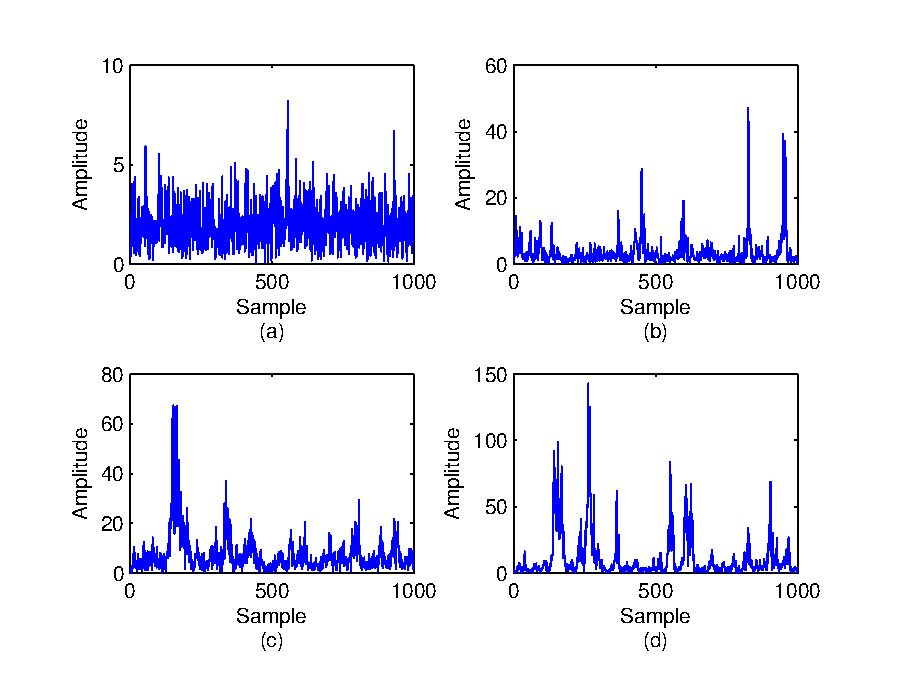
\includegraphics[width=0.75\textwidth]{figures/Fig_1_1.eps}
 \caption{**结果}\label{fig:diagram}
\end{figure}


\subsection{***研究进展}
\esubsection{Research progress}

%\label{sec:requirements}
首例***是**公司开发成功的……。

\subsection{****}
\esubsection{***}


*****************\cite{Jiang2005Size} ,如表 \ref{tab:category}所示。

\begin{table}
  \centering
  \caption{*****} \label{tab:category}
  \begin{tabular*}{0.9\textwidth}{@{\extracolsep{\fill}}cccc}
  \toprule
    1			&2		&3		&5 \\
  \midrule
    甲			&乙	    &丙		&丁 \\
    子		    &丑		&寅  	&某\\
  \bottomrule
  \end{tabular*}
\end{table}

********。
……

